\documentclass[conference]{IEEEtran}
\usepackage{graphicx}
\usepackage{hyperref}
\usepackage{balance}

\title{Avaliação de Modelos de IA Generativa para Documentação Automática de Código}
\author{
    \IEEEauthorblockN{Seu Nome}
    \IEEEauthorblockA{\textit{Departamento de Ciência da Computação} \\
    \textit{Universidade XYZ}\\
    Cidade, País \\
    email@dominio.com}
}

\begin{document}

\maketitle

\begin{abstract}
Este trabalho avalia modelos de IA generativa...
\end{abstract}

\section{Introdução}
A documentação de código é um...

\section{Fundamento Teórico}
\subsection{IA Generativa}
Modelos como GPT-4 \cite{gpt4}...

\section{Metodologia}
\begin{figure}[!t]
\centering
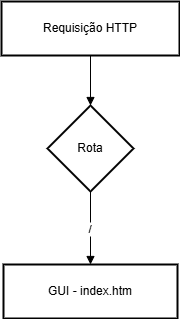
\includegraphics[width=3in]{figures/workflow.png}
\caption{Fluxo de trabalho proposto}
\label{fig_workflow}
\end{figure}

\section{Resultados}
\begin{table}[!t]
\caption{Comparação de Modelos}
\label{table_results}
\centering
\begin{tabular}{|c|c|c|c|}
\hline
Modelo & BLEU & ROUGE-1 & Tempo (s)\\
\hline
GPT-4 & 0.82 & 0.78 & 2.3\\
Llama & 0.65 & 0.62 & 1.8\\
Claude & 0.75 & 0.71 & 2.1\\
Gemini & 0.78 & 0.74 & 2.5\\
\hline
\end{tabular}
\end{table}

\balance
\bibliographystyle{IEEEtran}
\bibliography{references}

\end{document}
